\documentclass[12pt]{article}

\usepackage{fontawesome}
\usepackage{hyperref}
\usepackage{xurl}
\usepackage{graphicx}
\usepackage{float}
\usepackage[tagged, highstructure]{accessibility}
\usepackage{bookmark}
\usepackage{enumitem}

\hypersetup{
    colorlinks=false,
    pdfborder={0 0 0},
    pdftitle={Malware Analysis},
    pdfauthor={Adrianna Holden-Gouveia},
    pdfsubject={Information Security - Lab Assignment},
    pdflang={en-US},
    pdfkeywords={malware, virus, Stuxnet, WannaCry, security incidents, mitigation}
}

% Configure PDF bookmarks for navigation
\bookmarksetup{
    numbered,
    open,
}

% Configure list spacing for better accessibility
\setlist{nosep}



\title{Malware Analysis}
\author{
        Adrianna Holden-Gouveia \\
        Website: \href{https://aholdengouveia.name}{aholdengouveia.name}\\ 
        \date{\vspace{-5ex}}
        %Email: \href{mailto:admin@aholdengouveia.name}{admin@aholdengouveia.name} \\
%        \faLinkedin{: aholdengouveia} \\
        \faGithub {: aholdengouveia} \\
        \faTwitter {: aholdengouveia} \\
        }

%S\date{\today}


\begin{document}    

\maketitle

\section*{Accessibility Notice}
This document is also available in HTML format at:

Link: \href{https://aholdengouveia.name/InfoSec/labs/malwareanalysis.html}{\textbf{\nolinkurl{https://aholdengouveia.name/InfoSec/labs/malwareanalysis.html}}}

The HTML version provides enhanced accessibility features including keyboard navigation, screen reader support, responsive design, dark mode support, and high contrast options.


%\begin{abstract}
%This is a template for Linux Administration Lab work
%\end{abstract}
%\tableofcontents

\section*{Learning Outcomes}
By the end of this lab, you will be able to:
\begin{itemize}
    \item Explain how past malware incidents happened, what they caused, and the lessons learned
    \item Analyze a recent malware attack, including its attack vector, behavior, targets, and impact
    \item Recommend ways to prevent and reduce malware infections, and explain why they work
    \item Evaluate sources with the CRAAP test, and show that each one is real
\end{itemize}

\section*{Lab Instructions}
You'll write a report of at least 3 and a half pages about malware: two historical incidents, one recent attack, and your recommendations for preventing infections.

\subsection*{What your report must include}
Your report must be at least 3 and a half pages, not counting citations, checklists, or screenshots. Include these sections, clearly labelled:
\begin{enumerate}
    \item \textbf{Two historical malware incidents}, about 1 page each: two incidents that had a big impact on security or society, such as Stuxnet or WannaCry. For each one, explain how it happened, its consequences, and the lessons learned. Also say what type of malware it was, such as a virus, worm, trojan, rootkit, or ransomware, and explain how you decided.
    \item \textbf{A recent malware attack}, about 1 page: an attack from the last 2 years. Explain the attack vector, how the malware behaved, who or what it targeted, and its impact on the people, organizations, or governments affected. Also say what type of malware it was, and explain how you decided.
    \item \textbf{Recommendations}, about half a page: best practices for preventing and reducing malware infections, such as antivirus software, network security, and user education. Explain why each one helps.
    \item \textbf{Putting it into practice}: explain how your recommendations would apply to your own devices, your school, or a workplace you know. Be specific.
\end{enumerate}

\textbf{Malware types:} for all 3 of your malware examples, decide the type based on how it spread and what it did. For example, a worm spreads on its own, and a trojan hides inside a program that looks safe. Some malware is more than one type. WannaCry was ransomware that spread like a worm, so name every type that fits. Back up each choice with a source that describes the malware that way, and cite it in the sentence.

\subsection*{Sources}
You need at least 5 sources, including at least one dated source about your recent attack. For \textbf{each} source, include:
\begin{enumerate}
    \item A citation, in APA or MLA style. If you want to use another style, check with me first.
    \item A CRAAP test checklist or paragraph: Currency, Relevance, Authority, Accuracy, and Purpose.
    \item A screenshot of the source, showing its title and date.
    \item One direct quote from the source, and where it appears, such as the paragraph, section, or page.
\end{enumerate}
Citing in your report:
\begin{itemize}
    \item Anything you copy word for word is a quote. Put it in quotation marks and cite it.
    \item Anything you reword, or take the ideas from, still needs a citation.
    \item Ideas you've put together from several sources in your own words don't need a citation in the sentence, but the sources must be in your source list.
\end{itemize}

\subsection*{Screenshots}
Each screenshot should have your name, term, and year.  One of the easiest ways to do that is make a text document with your name and term/year on your computer and save it to use all term. Any screenshots that don't include this information won't be counted.

\begin{figure}[H]
    \centerline{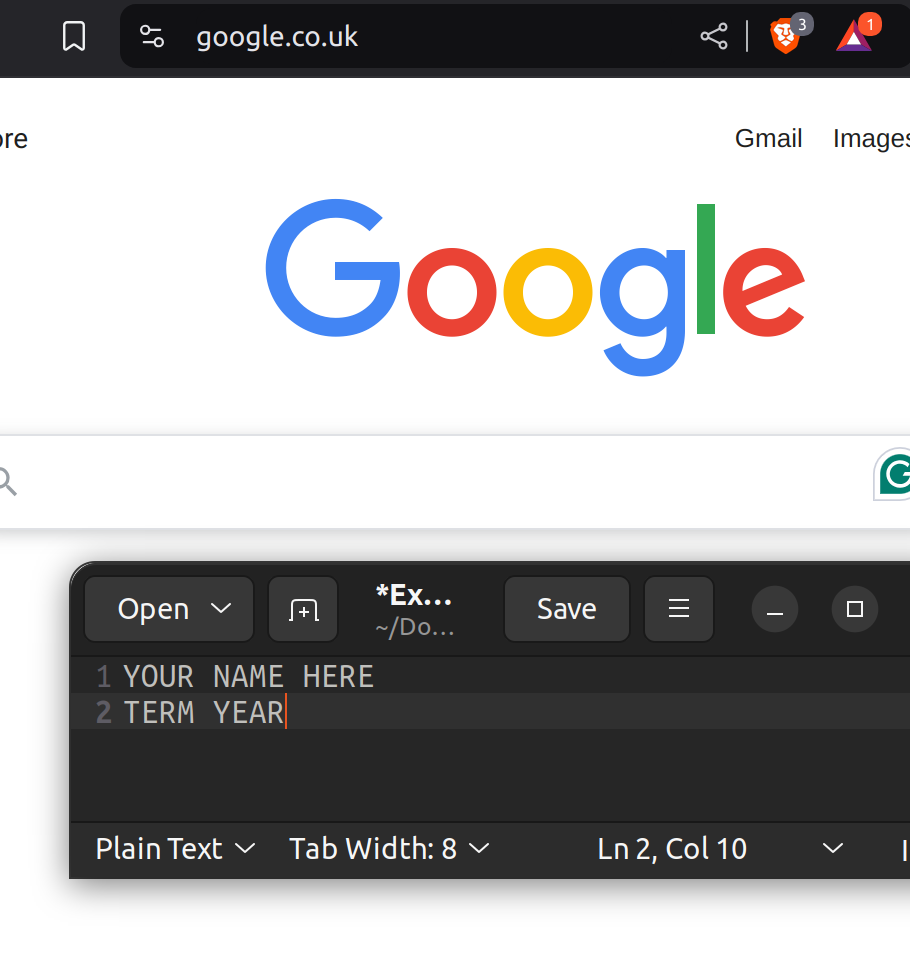
\includegraphics[scale=.2]{ExampleScreenshot.png}}
    \caption{This is an image of what each of your screenshots should look like}
    \alt{Example screenshot: a web browser showing the Google home page, with a small text editor window in front of it that says YOUR NAME HERE and TERM YEAR}
\end{figure}

\section*{Deliverables}
One file that includes:
\begin{itemize}
    \item Your report, with all 4 sections clearly labelled
    \item Your source list, with a CRAAP check, a screenshot, and a direct quote for each source
\end{itemize}
The CRAAP checks, screenshots, and quotes can go at the end of your report.

\section*{Resources}
References, a video, a PowerPoint and some notes are available at my website
Link: \href{https://www.aholdengouveia.name/InfoSec/Malware.html}{\textbf{\nolinkurl{https://www.aholdengouveia.name/InfoSec/Malware.html}}}

My guide to evaluating sources
Link: \href{https://www.aholdengouveia.name/Howtos/Sourceeval/sourceEvaluation.html}{\textbf{\nolinkurl{https://www.aholdengouveia.name/Howtos/Sourceeval/sourceEvaluation.html}}}

The CRAAP test, with questions to ask about each source
Link: \href{https://web.archive.org/web/20250814000638/https://guides.lib.uchicago.edu/c.php?g=1241077&p=9082343}{\textbf{\nolinkurl{https://web.archive.org/web/20250814000638/https://guides.lib.uchicago.edu/c.php?g=1241077&p=9082343}}}

Another explanation of the CRAAP test
Link: \href{https://libguides.butler.edu/c.php?g=117303&p=1940068}{\textbf{\nolinkurl{https://libguides.butler.edu/c.php?g=117303&p=1940068}}}

\end{document}